% Made up for the tikra benchmark.
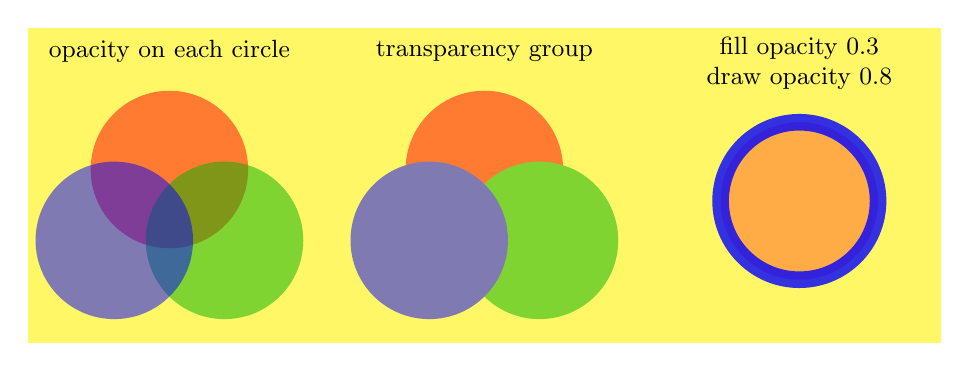
\begin{tikzpicture}
  \fill[yellow!60] (-1.8,-1.8) rectangle (9.8,2.2);
  % left: each circle at half opacity, the overlaps show darker
  \begin{scope}[opacity=0.5]
    \fill[red] (0,0.4) circle (1);
    \fill[green!70!black] (0.7,-0.5) circle (1);
    \fill[blue] (-0.7,-0.5) circle (1);
  \end{scope}
  \node[font=\small] at (0,1.9) {opacity on each circle};
  % right: one group at half opacity, the overlaps do not add up
  \begin{scope}[xshift=4cm, transparency group, opacity=0.5]
    \fill[red] (0,0.4) circle (1);
    \fill[green!70!black] (0.7,-0.5) circle (1);
    \fill[blue] (-0.7,-0.5) circle (1);
  \end{scope}
  \node[font=\small] at (4,1.9) {transparency group};
  % fill and draw opacity apart
  \draw[line width=6pt, draw=blue, fill=red, fill opacity=0.3, draw opacity=0.8] (8,0) circle (1);
  \node[font=\small, align=center] at (8,1.75) {fill opacity 0.3\\ draw opacity 0.8};
\end{tikzpicture}
